\documentclass[12pt,a4paper]{article}
\usepackage[T1]{fontenc}
\usepackage[utf8]{inputenc}
\usepackage[margin=25mm]{geometry}
\usepackage{graphicx,booktabs,amsmath,array,microtype,xcolor}
\usepackage[labelfont=bf,font=small]{caption}
\usepackage[hidelinks]{hyperref}
\usepackage{float,fancyhdr}
\setlength{\parindent}{0pt}
\setlength{\parskip}{5pt plus 1pt}
\fancyhf{}\fancyfoot[C]{\thepage}\renewcommand{\headrulewidth}{0pt}\pagestyle{fancy}
\begin{document}
\begin{center}
{\Large\bfseries Pool-ball Detection and Recognition}\\[3pt]
Manon Yiqin Galian Ng (23375206) -- CSU44053
\end{center}

\section{Overview}
The objective of this project was to locate pool balls in photographs of a table
and identify each ball by type and number. I divided the task into detecting
candidate balls and recognising their identities, then converted their positions
into table coordinates for the final views. 
% Development was iterative: I began with simple approaches and used intermediate
% images and quantitative errors to decide what to change. AllBalls supplied tuning
% and colour references; Tables1--6 supported evaluation and refinement.

\begin{figure}[H]\centering
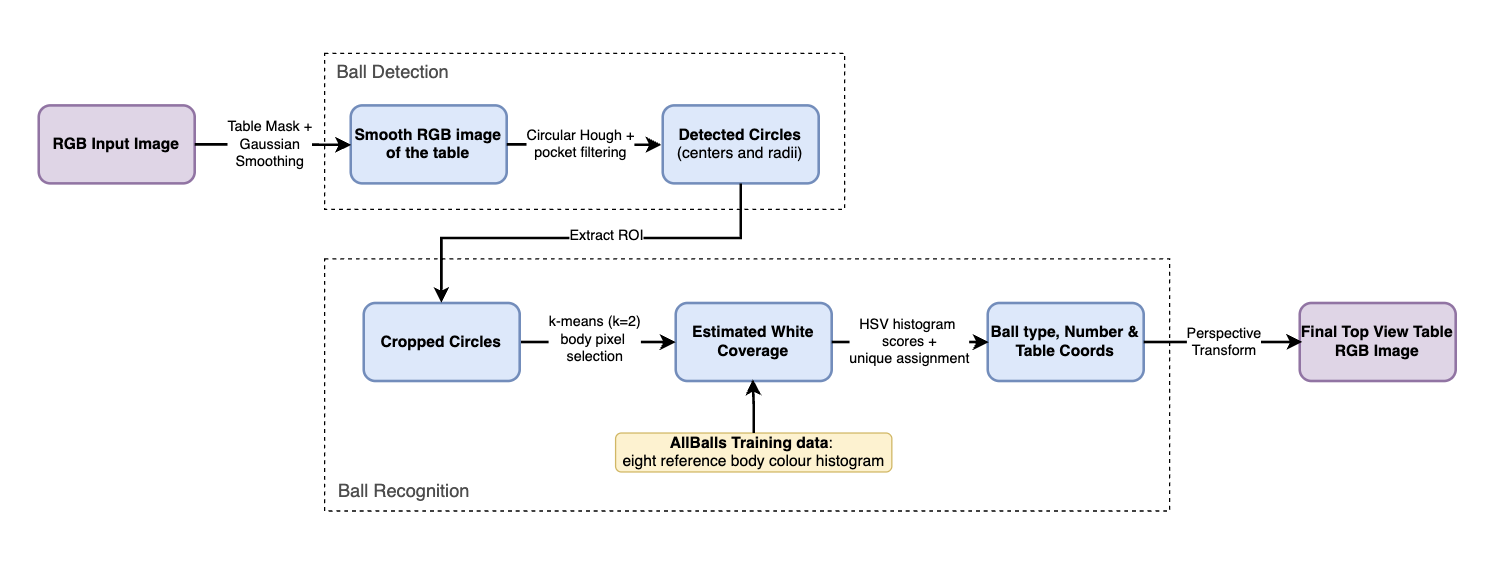
\includegraphics[width=.76\linewidth,trim=18bp 32bp 18bp 25bp,clip]{assets/pipeline.png}
\caption{Diagram of the Final Pipeline}
\end{figure}

\section{Detailed Design}
\subsection{Ball Detection}
I used the supplied corners to create a mask of the playing surface
and set the background to black.
I then converted the image to greyscale and smoothed it with a $5\times5$ Gaussian filter ($\sigma=1.5$) to reduce small
intensity variations before circular Hough transform.

% SOURCE: full saved masked and smoothed AllBalls images.
\noindent\begin{minipage}{\linewidth}\centering
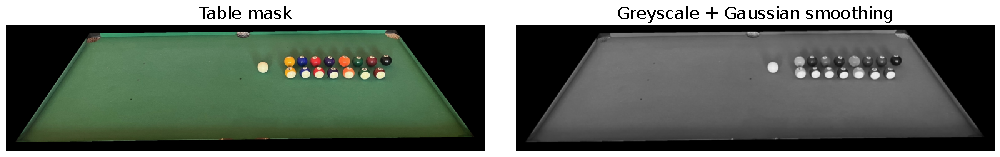
\includegraphics[width=\linewidth]{assets/detection_preprocessing.pdf}
\captionof{figure}{Masking (left) and greyscale smoothing (right) on AllBalls.}
\end{minipage}

I initially varied Hough parameters manually on AllBalls. This was slow and configurations were hard to compare, so I searched and evaluated 480 configurations.
The centers were matched to annotations in table coordinates. I ranked settings by
highest number of correct detections (missed ball cannot be recognised later) then by fewest 
extras and finally by lowest centre error (smallest average distance between detected and annotated ball centres).

% SOURCE: full saved starting/tuned raw Hough frames and tuned filtered result.
\noindent\begin{minipage}{\linewidth}\centering
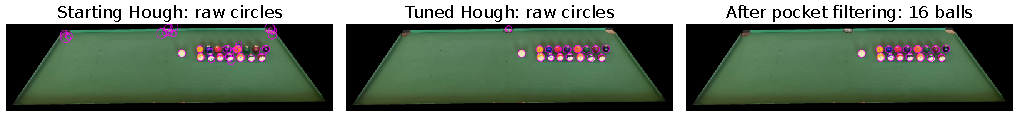
\includegraphics[width=\linewidth]{assets/hough_comparison.pdf}
\captionof{figure}{Starting Hough (left), tuned Hough (centre) and pocket filtering (right).}
\end{minipage}

% The final selected parameters are as follows: accumulator resolution ratio of 1.5, centre separation 18 pixels,
% upper Canny threshold of 75 and circle-centre accumulator threshold 35, with a fixed radius range of 15--30 pixels.
% Pockets sometimes produced circles. So balls with centers within 25 table units of pockets were filtered out.
% This left all 16 balls from 17 AllBalls circles, but there could be risk of
% removing genuine balls beside pockets.

% The final selected parameters are as follows. The gradient-based Hough method includes Canny 
% internally. We selected an upper threshold of 75 was the lowest tested, 
% allowing weaker edges to contribute, while the accumulator threshold of 
% 35 rejected weak voting peaks. The 18-pixel centre separation was below 
% the minimum accepted diameter of 30 pixels, keeping closely spaced 
% detections eligible. An accumulator ratio of 1.5 reduced the voting 
% grid’s width and height to approximately two-thirds of the image 
% dimensions, while radii of 15–30 pixels restricted detection to the 
% expected ball scale.

The grid search selected an accumulator ratio of 1.5, minimum centre 
separation of 18 pixels, upper Canny threshold of 75 and centre-accumulator
threshold of 35. Radii were fixed at 15–-30 pixels.

Since the Hough method already includes Canny, a separate edge-detection step was not needed. 
The lower Canny threshold allowed weaker edges to be used, while the accumulator threshold 
required enough votes before accepting a centre. The minimum centre distance reduced duplicate 
detections without excluding nearby balls. A ratio of 1.5 used a smaller grid to count votes, 
saving memory but making centre positions less precise.

Finally, each detected candidate was extracted as a square centred on its location, with
side length $2r+1$. A circular mask excluded the square's corner pixels. Keeping
the original colours and mask allowed me to compare recognition approaches on
the same crop and inspect individual mistakes.

\subsection{Ball Type Recognition}
I separated recognition into estimating type and body colour. My first type
estimator used HLS lightness and saturation to count white, dark and coloured
pixels inside each circle. The proportions then determined the type. But, reflections,
shadows and imperfect boundaries made these fixed thresholds unreliable: only
43/86 balls were typed correctly.

I then used K-means to separate light and coloured regions.
I initially chose \(k=2\) to reflect the light and coloured regions visible on 
pool balls, and retained it after testing other values on AllBalls because this simple 
grouping worked well.  
I then manually tested 
the cluster-classification thresholds, retaining \(V\ge170\) and \(S\le165\) for light; 
remaining clusters were dark if \(V\le90\), and coloured otherwise. The light-pixel fraction 
\(w\) determined type: at least 85\% light meant White, 
at least 70\% non-light meant Solid, and other mixtures meant Striped. This improved type 
recognition to 76/86. Higher \(k\) could separate shadows and reflections into additional 
clusters, but would need further evaluation.

% SOURCE: actual AllBalls cue/solid/stripe crops, cluster masks and measured areas.
\begin{figure}[H]\centering
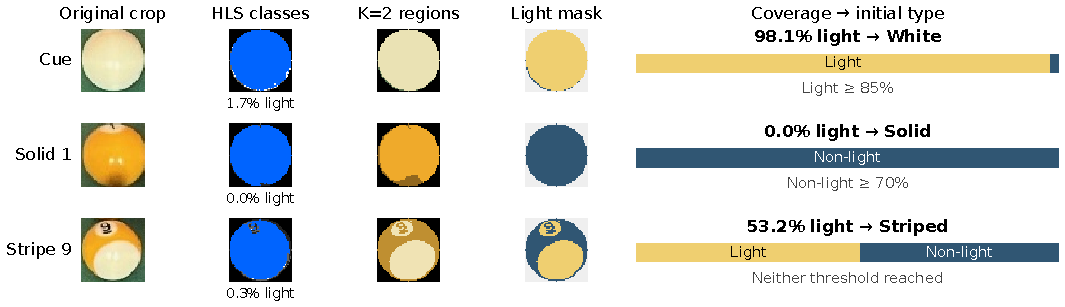
\includegraphics[width=.96\linewidth]{assets/type_development.pdf}
\caption{AllBalls cue, solid and stripe examples for HLS and $k$ means}
\end{figure}

\subsection{Ball Colour Recognition}
I first applied HSV threshold rules to the mean colour of the largest non-light K-means cluster. 
But shadows and reflections could distort this single average, so I switched to histograms to preserve the different 
body colours and their proportions.

I built eight references by grouping labelled AllBalls crops by body colour,
pairing solids and stripes. Black is always solid and the cue was excluded. I eroded
each circular mask with a $3\times3$ ellipse and removed pixels with $V\ge170$,
$S\le165$. This reduced cloth contamination, shared white stripes, patches
and highlights that could make different colours look alike.

For histogram resolutions I selected 18 hue bins and 8 bins each for saturation 
and brightness, balancing colour discrimination with the limited number of pixels 
available in each ball crop.
I smoothed neighbouring bins with $[1,2,1]/4$ along each axis, wrapping hue. Nearly neutral pixels
(BGR range below 15) received hue zero.

I normalised each crop's histogram to sum to one before averaging colour partners,
giving both equal influence despite different body-pixel counts. Fewer than 12
body pixels gave an Unknown colour label.

\begin{figure}[H]\centering
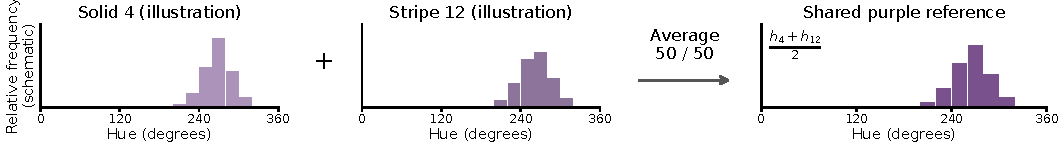
\includegraphics[width=.96\linewidth]{assets/reference_construction.pdf}
\caption{Approximate histogram reference example on purple balls}
\end{figure}

Finally, each candidate's body-colour histogram were compared with all eight references using one minus Bhattacharyya
distance to give similarity $s_{i,c}$ scores. The inital k means approach gave 65/80 
and the histogram with the representative-colour rules improved the results to 73/80 with 8
corrections and no regression.

% SOURCE: native ROI exports and ball_colours/hard_hue CSVs.
\begin{figure}[H]\centering
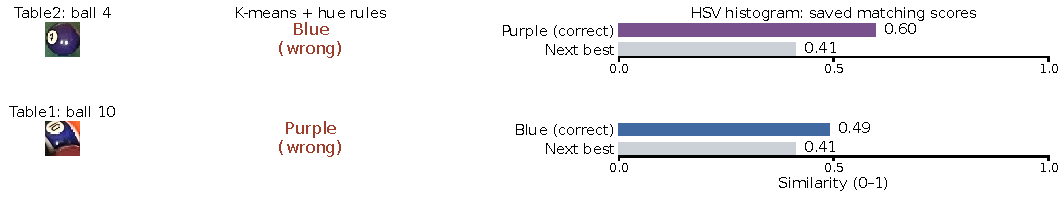
\includegraphics[width=.96\linewidth]{assets/colour_comparison.pdf}
\caption{Exported results (csv \& ball crops) show two colour corrections.}
\end{figure}

\subsection{Soft Score Approach}

Then, a property I wanted to leverage was that each ball has a unique identity. To use this I pivoted to soft scores
instead of hard decisions. Therefore, I first replace the single type 
classification with compatibility scores for Solid, Striped and Cue. 
I kept the original light-coverage intervals that were previously used: \([0,0.30]\) 
for Solid, \([0.30,0.85]\) for Striped and \([0.85,1]\) for White. A type received a score of 
one inside its interval, with support decreasing gradually outside it: $g_t(w)=\exp\!\left[-\frac{d(w,I_t)^2}{2(0.10)^2}\right]$

% $\quad \quad \quad \quad \quad \quad \quad \quad \quad \quad \quad \quad \quad \quad g_t(w)=\exp\!\left[-\frac{d(w,I_t)^2}{2(0.10)^2}\right]$

%CHANGE this part is not great
% Here $d(w,I_t)$ is distance to the interval, with zero inside it. The Gaussian
% fall-off shares the RBF form \cite{rbf}, while full support within an interval
% matches Gaussian combination membership \cite{gauss2mf}. I chose width 0.10
% heuristically; these are compatibility scores, not calibrated probabilities.

Here \(d(w,I_t)\) is the distance from light coverage \(w\) to the type’s interval, 
with zero distance inside it. I used a Gaussian fall-off so small deviations beyond 
a boundary retained strong support, while larger deviations were penalised more heavily 
\cite{rbf,gauss2mf}. This kept plausible alternatives available for unique assignment. 
I chose the width \(0.10\) (ten percentage points) heuristically. It should be noted that these scores measured 
compatibility, not probability.

For numbered balls, I multiplied histogram colour similarity by type compatibility: 
\(S_{i,n}=s_{i,c(n)}g_{t(n)}(w_i)\). The cue instead used \(S_{i,0}=w_i g_{\mathrm{White}}(w_i)\),
rewarding high light coverage and adding a penalty below 85\%. 
These scores provided the alternatives needed for the unique assignment stage.

\subsection{Unique identity assignment Algorithm}
To enforce uniqueness, I used the Hungarian algorithm \cite{hungarian} to maximise the total compatibility score 
across the table. Each row of the score matrix represented a candidate and each column a possible 
identity. The algorithm built an assignment while allowing earlier pairings to be rearranged, 
selecting one identity per candidate and using each identity at most once.

\begin{table}[H]
\centering
\begin{tabular}{lrrr}
\toprule
Table2 crop & Score for 4 & Score for 12 & Assigned identity \\
\midrule
Purple solid  & \textbf{0.597} & 0.128          & 4  \\
Purple stripe & 0.639          & \textbf{0.637} & 12 \\
\bottomrule
\end{tabular}
\caption{Scores example; the two purple crops in Table2}
\end{table}
In the table, both crops independently preferred 4. However, assigning the stripe to 12 barely reduced its score, 
whereas assigning the solid to 12 caused a much larger loss. The selected pairing therefore scored 
1.234 overall, compared with 0.767 for the reverse pairing.

Each detection also had an Unknown option, allowing surplus or ineligible candidates to 
remain unassigned. However, Unknown had a near-zero score, so even a weak match could 
receive an unused identity. This favoured assigning labels wherever possible, but offered 
limited rejection of false detections. Across Tables1–6, this approach improved correct 
identities from 73/86 to 75/86.

\begin{figure}[H]\centering
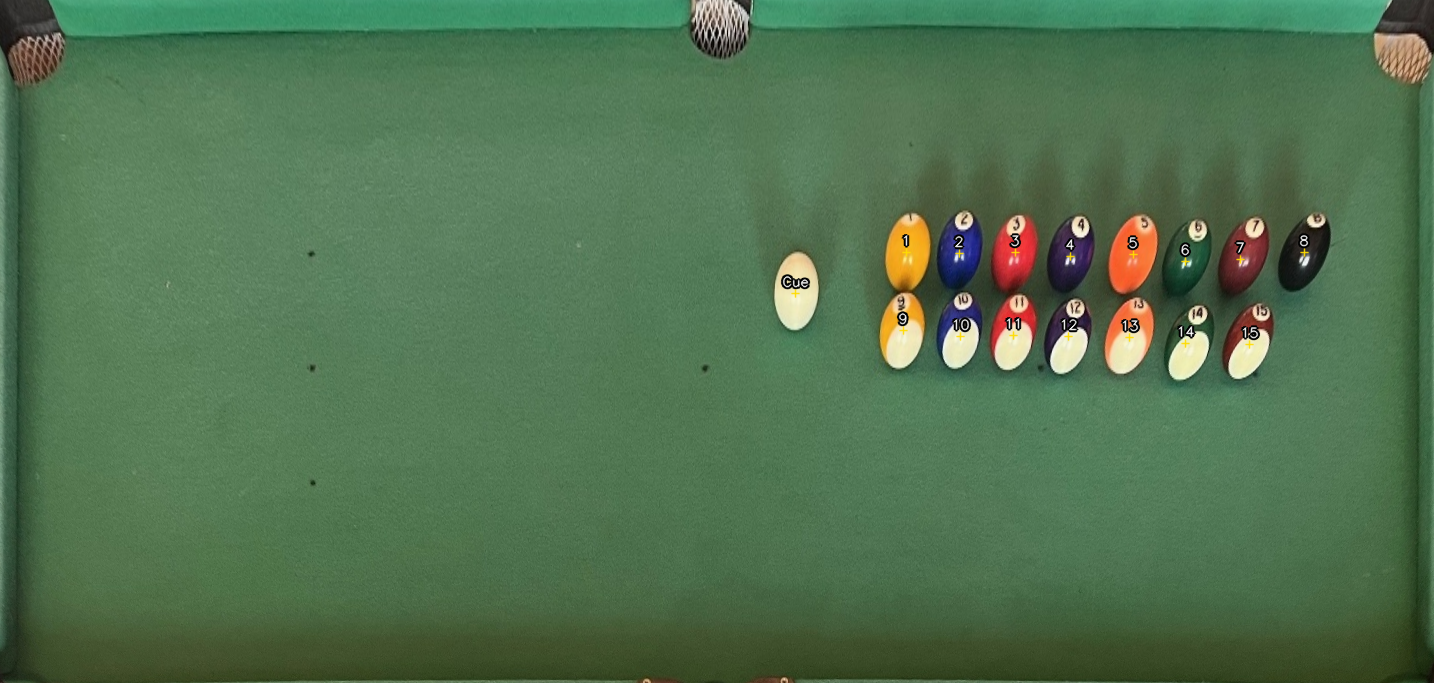
\includegraphics[width=.50\linewidth,trim=740bp 300bp 75bp 205bp,clip]{../final_output/final/AllBalls/table_numbered.png}
\caption{Cropped overhead view of AllBalls after recognition and perspective correction. AllBalls supplied tuning and colour references.}
\end{figure}

\subsection{Resolving cue-ball ambiguity}
Inspection revealed that Hough sometimes found the white patch inside the ball instead of the
full ball boundary. Several candidates could then appear White, and uniqueness
alone could give the cue to the wrong one. I introduced two refinements to resolve these issues.

First, I expanded the radius of originally White crops by one pixel, which performed best among the padding sizes tested, and recomputed
their type and colour evidence. 
This could recover a thin rim of body colour when detection captured mainly a white patch.
The stored centre and original detected radius
were unchanged. This improved correct
identities from 75/86 to 79/86.

Second, when several original candidates remained classified as White, I reserved the cue for the
largest original radius. A full ball should usually exceed a patch: Table1's
radii were 24.15 and 17.55 pixels. This improved performance to 80/86.  A more sophisticated approach could account for perspective by 
comparing each candidate’s radius with the expected apparent ball radius at its position on the 
table.

\noindent\begin{minipage}{\linewidth}\centering
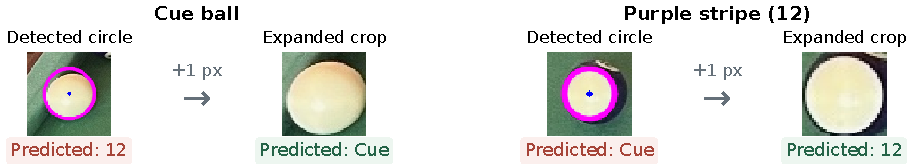
\includegraphics[width=.98\linewidth]{assets/cue_refinement.pdf}
\captionof{figure}{Table3: one-pixel radius expansion corrects the swapped cue and stripe-12 predictions.}
\end{minipage}

\section{Results and Analysis}
\subsection{Evaluation methodology}
I evaluated detection and recognition separately to distinguish missed balls from incorrect 
identities. For detection, I matched predicted centres to annotated positions in the 
perspective-corrected table, allowing a maximum Euclidean distance of 15 table units. Matching 
found as many valid pairs as possible, using each detection and annotation only once. Matched 
pairs counted as true positives (TP), extra detections as false positives (FP), and missed balls 
as false negatives (FN).

The 15-table-unit matching tolerance was a fixed heuristic, approximately one-third of the 
assumed 43-unit ball diameter. It allowed some uncertainty in detection and annotation while 
requiring the predicted centre to remain within the ball’s nominal radius.

Precision, $\mathrm{TP}/(\mathrm{TP}+\mathrm{FP})$, measured how many detections
corresponded to real balls. Recall, $\mathrm{TP}/(\mathrm{TP}+\mathrm{FN})$,
measured how many annotated balls were found. F1 combined them as
$2\mathrm{TP}/(2\mathrm{TP}+\mathrm{FP}+\mathrm{FN})$.
Mean localisation error measured the average centre-to-centre distance of matched pairs using
$\mathrm{MLE}=\frac{1}{N}\sum_{i=1}^{N}
\sqrt{(x_i-\hat{x}_i)^2+(y_i-\hat{y}_i)^2}$.

Recognition accuracy measured the fraction of matched balls given the correct
identity. End-to-end accuracy divided correct identities by all annotated balls,
so missed balls also counted as failures. Unknown labels counted as incorrect.
False detections reduced precision but were excluded from these recognition
fractions. Body-colour accuracy excluded the cue.

I reported AllBalls separately because it supplied tuning and colour references.
The pooled results cover Tables1--6, which also guided development. They therefore
describe performance on images used to refine the system, rather than an independent test.

\subsection{Final Metrics}
The final system detected 86 of the 90 annotated balls, with two false positives.
Precision was \textbf{97.73\%}, recall \textbf{95.56\%} and F1 \textbf{96.63\%}.
Mean centre error was 4.91 table units across the 86 matches. Of those matched
balls, \textbf{80/86} had the correct identity (\textbf{93.02\%}), giving
\textbf{80/90}, or \textbf{88.89\%}, end-to-end accuracy.

I also compared performance for each ball identity to see which balls were recognised reliably and which caused the most errors.
\begin{figure}[H]\centering
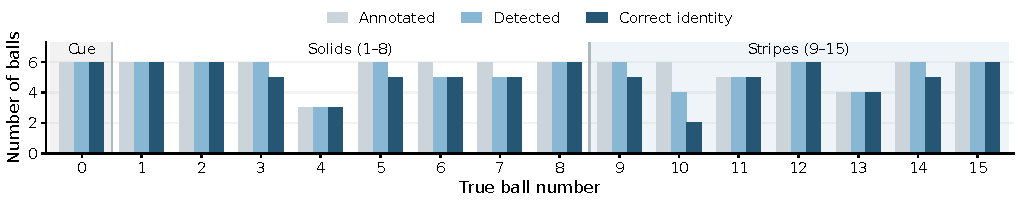
\includegraphics[width=.96\linewidth]{assets/identity_counts.pdf}
\caption{Counts by true identity on Tables1--6 (0 is the cue). Correct identities:
solids 41/45, stripes 33/39, cues 6/6.}
\end{figure}

\subsection{Final Table Views}

Using the four supplied corners, I calculated a perspective transform that mapped the playing 
surface to a \(1434\times683\) rectangle, then applied the same transform to the detected ball 
centres. The warping was done post detection and recognition so as to not affect the ball shapes.

% SOURCE: unchanged saved table_numbered.png/table_diagram.png pairs for all six tables.
\begin{figure}[H]\centering
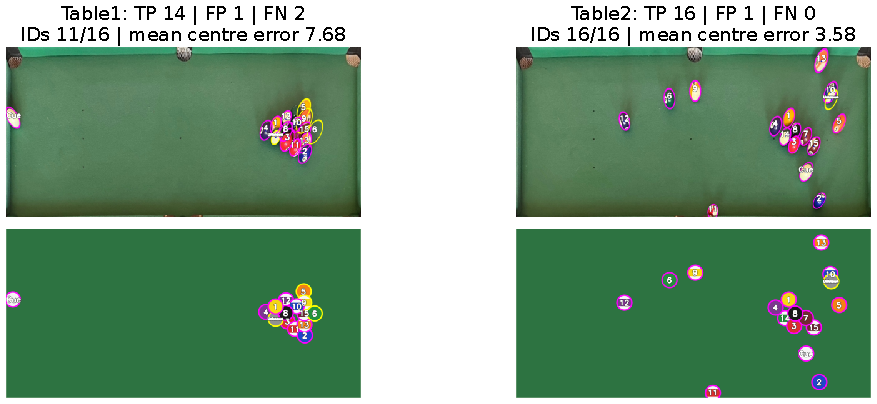
\includegraphics[width=.98\linewidth]{assets/final_views_1_2.pdf}
\phantomcaption
\end{figure}

\begin{figure}[H]\ContinuedFloat\centering
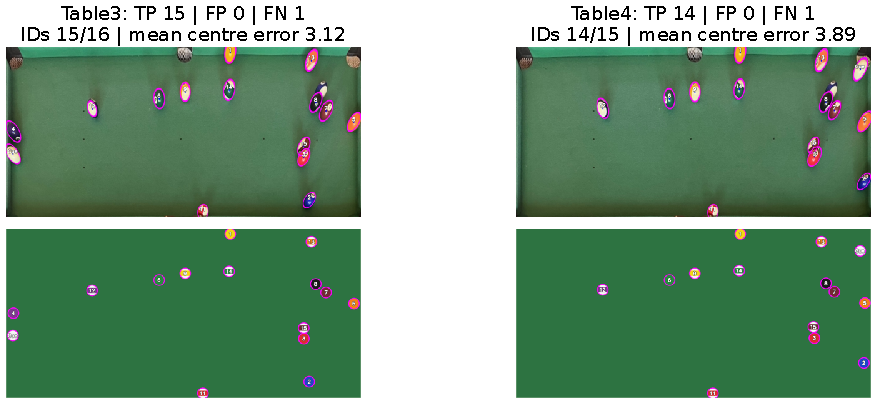
\includegraphics[width=.98\linewidth]{assets/final_views_3_4.pdf}
\end{figure}

\begin{figure}[H]\ContinuedFloat\centering
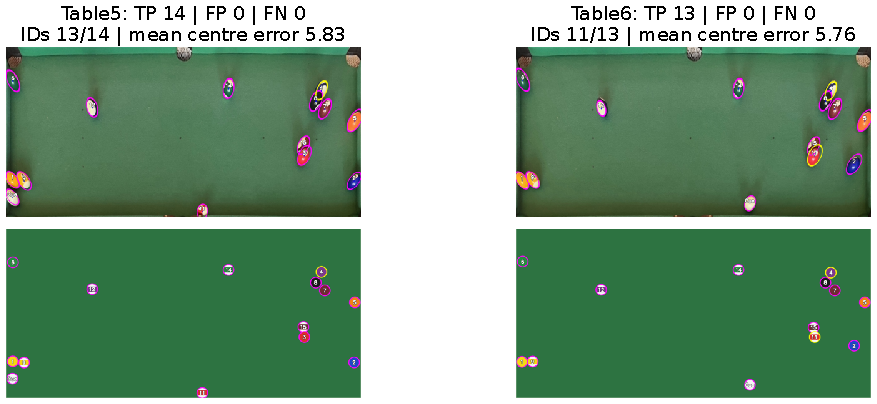
\includegraphics[width=.98\linewidth]{assets/final_views_5_6.pdf}
\caption[]{Final visulisation for Tables1--6.}
\end{figure}

The final views pair a numbered rectified photograph with an overhead diagram. The photograph 
shows the predictions in context, while the diagram uses enlarged markers for readability.
Magenta outlines indicate correct identities while yellow indicates wrong identities or false circles, 
using annotations only for these evaluation colours.

\subsection{Observed Strengths and Weaknesses}
Table2 was the clearest success: all 16 real balls were correctly identified, while the extra 
circle remained Unknown. The system could therefore handle some ambiguous appearances and an 
additional detection without losing correct identities. Tables3 and 4 also identified every 
detected ball correctly, although both missed ball 10. In these cases, detection was the remaining 
obstacle to a completely correct result.

Table1 exposed the limits of circle detection in a crowded arrangement. Balls 6 and 7 were missed, 
a false circle received identity 6, and balls 5 and 9 exchanged labels. The exchanged balls had 
centre errors of 14.63 and 14.81 table units, close to the 15-unit matching tolerance. They 
counted as successful detections, but their displaced crops could include neighbouring material 
or exclude part of the intended ball. A valid centre match therefore did not guarantee useful 
recognition evidence.

In Table1, the green stripe's crop captured mainly white, leaving too little green for matching.
One-pixel padding performed best overall among the sizes tested, but this ball
remained Unknown. Table6's blue stripe instead included a dark neighbour and was
labelled as a purple solid. Larger crops may recover missing colour, but can also
admit neighbours, so increasing padding alone cannot reliably resolve both errors.

Table6's red solid exposed a separate weakness. Its bright red surface passed the
light thresholds, inflating white coverage and producing a red-striped label
despite the correct body-colour match.

The system performed well overall, but the remaining errors show there is still room to improve detection and recognition.

% SOURCE: the same measured failure crops and selected-pixel/cluster views.
\begin{figure}[H]\centering
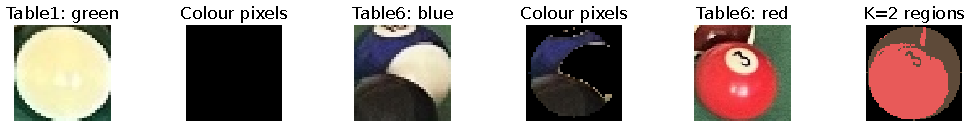
\includegraphics[width=.98\linewidth]{assets/failure_details.pdf}
\caption{Failure examples: context and detected circles above, crops and evidence below.
Gold marks pixels counted as light; black marks excluded pixels.}
\end{figure}

\subsection{Possible Next Steps \& Conclusion}
\label{sec:assessment}
The current type classifier uses k-means colour groups and their proportions, 
without considering their spatial arrangement. Connected-component analysis (CCA) 
could examine the size, position and connectivity of white and coloured regions, 
adding evidence to help distinguish solids from stripes.

For detection, guided Hough could focus circle searches on crowded regions using the 
expected ball size. Watershed could then use the candidate centres as markers to 
separate touching balls into individual regions. This could help recover missed balls and produce cleaner recognition crops containing less neighbouring material.

Additionally, we could test lighting correction to make white coverage estimates more 
accurate and consistent across different lighting conditions.

\textbf{Conclusion.} 
The pipeline performed well for the tested setup. AllBalls provided clear reference examples but 
limited variety, so the table images were needed to reveal edge cases such as overlapping balls 
and imperfect crops. These cases helped refine the general approach, while I aimed to limit 
adjustments for individual images. Additional fully unseen test images would help assess how 
well these refinements carry over to new arrangements and lighting conditions, with the parameters 
kept fixed.

\begin{thebibliography}{4}
\setlength{\itemsep}{2pt}
\bibitem{course} K. Dawson-Howe, \emph{CSU44053 Computer Vision course material},
Trinity College Dublin.
\bibitem{opencv}
OpenCV,
\href{https://docs.opencv.org/4.12.0/}
{\emph{OpenCV 4.12.0 Documentation}}
\bibitem{rbf} Scikit-learn Developers, \emph{User Guide}, \S1.7.4.3,
\href{https://scikit-learn.org/stable/modules/gaussian_process.html\#radial-basis-function-rbf-kernel}{``Radial basis function (RBF) kernel.''}
\bibitem{gauss2mf} MathWorks, \emph{Fuzzy Logic Toolbox documentation},
\href{https://www.mathworks.com/help/fuzzy/gauss2mf.html}{``Gaussian combination membership function.''}
\bibitem{hungarian} CP-Algorithms,
\href{https://cp-algorithms.com/graph/hungarian-algorithm.html}{``Hungarian Algorithm.''}
\end{thebibliography}

\textbf{Code Repository:} \url{https://github.com/galiannm/pool-ball-recogniser}
\end{document}